% Options for packages loaded elsewhere
% Options for packages loaded elsewhere
\PassOptionsToPackage{unicode}{hyperref}
\PassOptionsToPackage{hyphens}{url}
\PassOptionsToPackage{dvipsnames,svgnames,x11names}{xcolor}
%
\documentclass[
]{IEEEtran}
\usepackage{xcolor}
\usepackage{amsmath,amssymb}
\setcounter{secnumdepth}{5}
\usepackage{iftex}
\ifPDFTeX
  \usepackage[T1]{fontenc}
  \usepackage[utf8]{inputenc}
  \usepackage{textcomp} % provide euro and other symbols
\else % if luatex or xetex
  \usepackage{unicode-math} % this also loads fontspec
  \defaultfontfeatures{Scale=MatchLowercase}
  \defaultfontfeatures[\rmfamily]{Ligatures=TeX,Scale=1}
\fi
\usepackage{lmodern}
\ifPDFTeX\else
  % xetex/luatex font selection
  \setmonofont[Scale=0.60]{BigBlueTermPlus Nerd Font Mono}
\fi
% Use upquote if available, for straight quotes in verbatim environments
\IfFileExists{upquote.sty}{\usepackage{upquote}}{}
\IfFileExists{microtype.sty}{% use microtype if available
  \usepackage[]{microtype}
  \UseMicrotypeSet[protrusion]{basicmath} % disable protrusion for tt fonts
}{}
\makeatletter
\@ifundefined{KOMAClassName}{% if non-KOMA class
  \IfFileExists{parskip.sty}{%
    \usepackage{parskip}
  }{% else
    \setlength{\parindent}{0pt}
    \setlength{\parskip}{6pt plus 2pt minus 1pt}}
}{% if KOMA class
  \KOMAoptions{parskip=half}}
\makeatother
% Make \paragraph and \subparagraph free-standing
\makeatletter
\ifx\paragraph\undefined\else
  \let\oldparagraph\paragraph
  \renewcommand{\paragraph}{
    \@ifstar
      \xxxParagraphStar
      \xxxParagraphNoStar
  }
  \newcommand{\xxxParagraphStar}[1]{\oldparagraph*{#1}\mbox{}}
  \newcommand{\xxxParagraphNoStar}[1]{\oldparagraph{#1}\mbox{}}
\fi
\ifx\subparagraph\undefined\else
  \let\oldsubparagraph\subparagraph
  \renewcommand{\subparagraph}{
    \@ifstar
      \xxxSubParagraphStar
      \xxxSubParagraphNoStar
  }
  \newcommand{\xxxSubParagraphStar}[1]{\oldsubparagraph*{#1}\mbox{}}
  \newcommand{\xxxSubParagraphNoStar}[1]{\oldsubparagraph{#1}\mbox{}}
\fi
\makeatother

\usepackage{color}
\usepackage{fancyvrb}
\newcommand{\VerbBar}{|}
\newcommand{\VERB}{\Verb[commandchars=\\\{\}]}
\DefineVerbatimEnvironment{Highlighting}{Verbatim}{commandchars=\\\{\}}
% Add ',fontsize=\small' for more characters per line
\usepackage{framed}
\definecolor{shadecolor}{RGB}{241,243,245}
\newenvironment{Shaded}{\begin{snugshade}}{\end{snugshade}}
\newcommand{\AlertTok}[1]{\textcolor[rgb]{0.68,0.00,0.00}{#1}}
\newcommand{\AnnotationTok}[1]{\textcolor[rgb]{0.37,0.37,0.37}{#1}}
\newcommand{\AttributeTok}[1]{\textcolor[rgb]{0.40,0.45,0.13}{#1}}
\newcommand{\BaseNTok}[1]{\textcolor[rgb]{0.68,0.00,0.00}{#1}}
\newcommand{\BuiltInTok}[1]{\textcolor[rgb]{0.00,0.23,0.31}{#1}}
\newcommand{\CharTok}[1]{\textcolor[rgb]{0.13,0.47,0.30}{#1}}
\newcommand{\CommentTok}[1]{\textcolor[rgb]{0.37,0.37,0.37}{#1}}
\newcommand{\CommentVarTok}[1]{\textcolor[rgb]{0.37,0.37,0.37}{\textit{#1}}}
\newcommand{\ConstantTok}[1]{\textcolor[rgb]{0.56,0.35,0.01}{#1}}
\newcommand{\ControlFlowTok}[1]{\textcolor[rgb]{0.00,0.23,0.31}{\textbf{#1}}}
\newcommand{\DataTypeTok}[1]{\textcolor[rgb]{0.68,0.00,0.00}{#1}}
\newcommand{\DecValTok}[1]{\textcolor[rgb]{0.68,0.00,0.00}{#1}}
\newcommand{\DocumentationTok}[1]{\textcolor[rgb]{0.37,0.37,0.37}{\textit{#1}}}
\newcommand{\ErrorTok}[1]{\textcolor[rgb]{0.68,0.00,0.00}{#1}}
\newcommand{\ExtensionTok}[1]{\textcolor[rgb]{0.00,0.23,0.31}{#1}}
\newcommand{\FloatTok}[1]{\textcolor[rgb]{0.68,0.00,0.00}{#1}}
\newcommand{\FunctionTok}[1]{\textcolor[rgb]{0.28,0.35,0.67}{#1}}
\newcommand{\ImportTok}[1]{\textcolor[rgb]{0.00,0.46,0.62}{#1}}
\newcommand{\InformationTok}[1]{\textcolor[rgb]{0.37,0.37,0.37}{#1}}
\newcommand{\KeywordTok}[1]{\textcolor[rgb]{0.00,0.23,0.31}{\textbf{#1}}}
\newcommand{\NormalTok}[1]{\textcolor[rgb]{0.00,0.23,0.31}{#1}}
\newcommand{\OperatorTok}[1]{\textcolor[rgb]{0.37,0.37,0.37}{#1}}
\newcommand{\OtherTok}[1]{\textcolor[rgb]{0.00,0.23,0.31}{#1}}
\newcommand{\PreprocessorTok}[1]{\textcolor[rgb]{0.68,0.00,0.00}{#1}}
\newcommand{\RegionMarkerTok}[1]{\textcolor[rgb]{0.00,0.23,0.31}{#1}}
\newcommand{\SpecialCharTok}[1]{\textcolor[rgb]{0.37,0.37,0.37}{#1}}
\newcommand{\SpecialStringTok}[1]{\textcolor[rgb]{0.13,0.47,0.30}{#1}}
\newcommand{\StringTok}[1]{\textcolor[rgb]{0.13,0.47,0.30}{#1}}
\newcommand{\VariableTok}[1]{\textcolor[rgb]{0.07,0.07,0.07}{#1}}
\newcommand{\VerbatimStringTok}[1]{\textcolor[rgb]{0.13,0.47,0.30}{#1}}
\newcommand{\WarningTok}[1]{\textcolor[rgb]{0.37,0.37,0.37}{\textit{#1}}}

\usepackage{longtable,booktabs,array}
\usepackage{calc} % for calculating minipage widths
% Correct order of tables after \paragraph or \subparagraph
\usepackage{etoolbox}
\makeatletter
\patchcmd\longtable{\par}{\if@noskipsec\mbox{}\fi\par}{}{}
\makeatother
% Allow footnotes in longtable head/foot
\IfFileExists{footnotehyper.sty}{\usepackage{footnotehyper}}{\usepackage{footnote}}
\makesavenoteenv{longtable}
\usepackage{graphicx}
\makeatletter
\newsavebox\pandoc@box
\newcommand*\pandocbounded[1]{% scales image to fit in text height/width
  \sbox\pandoc@box{#1}%
  \Gscale@div\@tempa{\textheight}{\dimexpr\ht\pandoc@box+\dp\pandoc@box\relax}%
  \Gscale@div\@tempb{\linewidth}{\wd\pandoc@box}%
  \ifdim\@tempb\p@<\@tempa\p@\let\@tempa\@tempb\fi% select the smaller of both
  \ifdim\@tempa\p@<\p@\scalebox{\@tempa}{\usebox\pandoc@box}%
  \else\usebox{\pandoc@box}%
  \fi%
}
% Set default figure placement to htbp
\def\fps@figure{htbp}
\makeatother





\setlength{\emergencystretch}{3em} % prevent overfull lines

\providecommand{\tightlist}{%
  \setlength{\itemsep}{0pt}\setlength{\parskip}{0pt}}



 
\usepackage[]{biblatex}
\addbibresource{bibliography.bib}


\usepackage{dirtytalk}
\usepackage{tikz}
\usepackage{listings}
%\usepackage[cmintegrals]{newtxmath}
%\usepackage{bm}
\lstset{basicstyle=\ttfamily\tiny, breaklines=true}
\usetikzlibrary{positioning}
\tikzset{
  x=2.8em,
  y=2.8em,
}
%! TeX program = xelatex
%! TeX TS-program = xelatex
%! TeX root = ProgramaciónEvolutiva.tex
%%%%%%%%%%%%%%%%%%%%%%%%%%%%%%%%%%%%%%%%%%%%%%%%%%%%%%%%%%%%%%%%%%%%%%%%
% Define AntiqueWhite color
\definecolor{AntiqueWhite}{RGB}{250,235,215}
\definecolor{mypurple}{RGB}{104,020,108}
\setbeamercolor*{palette primary}{use=structure,fg=white,bg=mypurple}
\setbeamercolor{normal text}{fg=white, bg=black}
\setbeamercolor{tcolorbox text}{fg=white, bg=black}
\setbeamertemplate{navigation symbols}{}                              %
\newcommand{\colouredcircle}{%
  \tikz{\useasboundingbox (-0.2em,-0.32em) rectangle(0.2em,0.32em);
        \draw[ball color=PineGreen!7!Plum!90!Red,shading=ball,line width=0.03em] (0,0) circle(0.18em);}}
\newcommand{\colouredcircledis}{%
  \tikz{\useasboundingbox (-0.2em,-0.32em) rectangle(0.2em,0.32em);
        \draw[ball color=PineGreen!7!Plum!20!Black,shading=ball,line width=0.03em] (0,0) circle(0.18em);}}
\setbeamertemplate{itemize item}{\colouredcircle}
\setbeamercolor*{bibliography entry title}{fg=Yellow!80!White, bg=Black}
% Set beamer bibliography titles and numbers color to antique white
\setbeamercolor*{bibliography entry author}{fg=AntiqueWhite}
\setbeamercolor*{bibliography entry location}{fg=AntiqueWhite}
\setbeamercolor*{bibliography entry note}{fg=AntiqueWhite}
%% Numbering color to Pine Green
\setbeamercolor*{bibliography item}{fg=LimeGreen!80!White}
% Set beamer bibliography urls color to some magenta
\setbeamercolor*{bibliography entry url}{fg=Magenta}
% Captions color to rgba (0,255,0,1)
\definecolor{LimeGreen}{RGB}{0,255,0}
\setbeamercolor{caption name}{fg=LimeGreen}
%%%%%%%%%%%%%%%%%%%%%%%%%%%%%%%%%%%%%%%%%%%%%%%%%%%%%%%%%%%%%%%%%%%%%%%%
\usepackage{tikzpagenodes}
\setbeamertemplate{background canvas}{%
  \begin{tikzpicture}[inner sep=0pt,remember picture,overlay]
    \node at (current page.center) {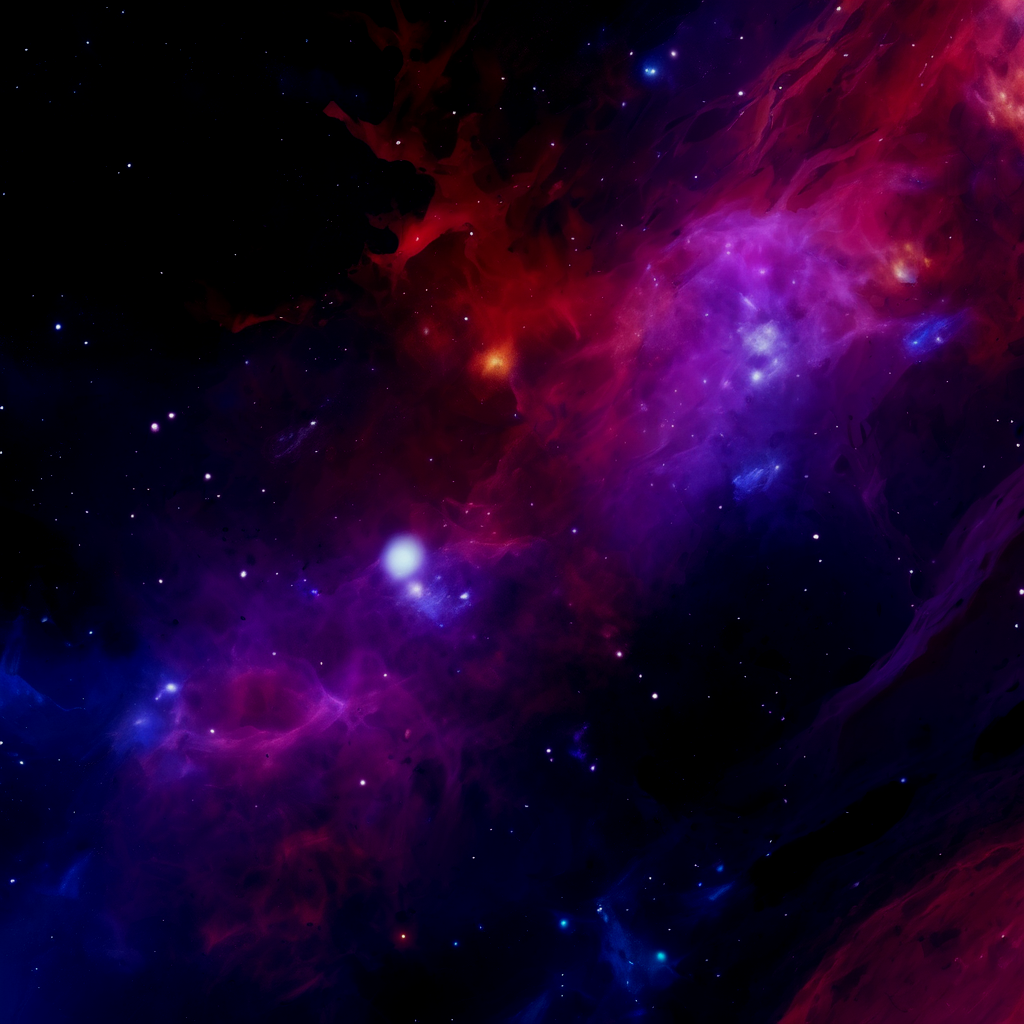
\includegraphics[height=\paperheight,width=\paperwidth]{fondo}};
  \end{tikzpicture}
}%
\usetikzlibrary{arrows.meta, decorations.pathmorphing,positioning,trees}

\lstset{
    basicstyle=\ttfamily\small,
    breaklines=true,
    backgroundcolor=\color{black!98},
    keywordstyle=\color{Magenta},
    commentstyle=\color{AntiqueWhite},
    stringstyle=\color{Yellow!80!white},
    showstringspaces=false,
    frame=single,
    rulecolor=\color{mypurple},
    frameround=tttt,
    escapeinside={\%*}{*)}
}

\makeatletter
% Set victor mono as default ttfont
\newtcolorbox{blur}[1][]{%
  #1,
  enhanced,
  remember,
  breakable, % Already enabled (good!)
  frame hidden,
  interior hidden,
  fonttitle=\bfseries\centering, 
  fontupper=\rmfamily\selectfont,
  coltext=white,
  underlay={
    \begin{tcbclipframe}
      \begin{scope}[inner sep=0pt,remember picture,overlay]
        \fill[white] (frame.south west) rectangle (frame.north east); % Changed to `frame` (not `current page`)
        \node[opacity=1] at (frame.center) {
\includegraphics[height=\paperheight, width=\paperwidth]{blured}};
      \end{scope}
    \end{tcbclipframe}
  }
}
\makeatother
%%%%%%%%%%%%%%%%%%%%%%%%%%%%%%%%%%%%%%%%%%%%%%%%%%%%%%%%%%%%%%%%%%%%%%%%
\newcommand{\separador}[1]{
  \vskip-4pt
  \begin{center}
    \rule{0.9\linewidth}{#1}
  \end{center}
}

\lstset{
  basicstyle=\ttfamily,
  showstringspaces=false,
  breaklines=true
}

\newcommand{\transparencia}[1]{%
  \begin{frame}
    \begin{blur}
      #1
    \end{blur}
  \end{frame}
}

% set bibliography background for text to be legible despite the background

\usepackage{etoolbox}
\newcommand{\setupblurbibliography}{%
  \pretocmd{\frametitle}{\blurbackground}{}{}%
  \setbeamertemplate{bibliography item}{\color{LimeGreen!80!White}\insertbiblabel}%
  \setbeamercolor{bibliography entry author}{fg=AntiqueWhite}%
  \setbeamercolor{bibliography entry title}{fg=Yellow!80!White}%
  \setbeamercolor{bibliography entry location}{fg=AntiqueWhite}%
  \setbeamercolor{bibliography entry note}{fg=AntiqueWhite}%
  \setbeamercolor{bibliography entry url}{fg=Magenta}%
}

\newtcblisting{beamerlst}[1][]{
    enhanced,
    breakable,
    listing only,
    listing options={
        style=beamerlisting,
        language=Python, % Default language
        #1
    },
    colback=black!85, % Matches your theme
    colframe=mypurple, % Your purple color
    fontupper=\ttfamily\small,
    arc=3mm, % Rounded corners
    boxrule=1pt,
    % Blur effect (optional):
    underlay={
        \begin{tcbclipframe}
        \fill[black!90] (frame.south west) rectangle (frame.north east);
        \node[opacity=0.6] at (frame.center) 
            {
\includegraphics[width=\linewidth]{blured}};
        \end{tcbclipframe}
    }
}

% Supporting style definition
\lstdefinestyle{beamerlisting}{
    basicstyle=\ttfamily\footnotesize\color{white},
    keywordstyle=\color{Magenta},
    commentstyle=\color{AntiqueWhite},
    stringstyle=\color{Yellow!80!white},
    showstringspaces=false,
    breaklines=true,
    tabsize=2
}

\newcommand{\codebox}[2][]{%
    \begin{tcolorbox}[
        enhanced,
        colback=black!85,
        colframe=mypurple,
        arc=3mm,
        boxrule=1pt,
        #1
    ]
    \lstinputlisting{#2}
    \end{tcolorbox}%
}

% Smart blur background that works with frame breaks
\newcommand{\blurbackground}{%
  \begin{tikzpicture}[remember picture,overlay]
    % Calculate content area with margins
    \path ([xshift=1cm,yshift=-1cm]current page.north west) coordinate (top left);
    \path ([xshift=-1cm,yshift=1cm]current page.south east) coordinate (bottom right);
    
    % Frosted glass effect
    \fill[black!85,opacity=0.92] (top left) rectangle (bottom right);
    \node[opacity=0.8] at (current page.center) 
      {
\includegraphics[width=\paperwidth-2cm,height=\paperheight-2cm]{blured}};
  \end{tikzpicture}%
}


\includeonly{01.-EvolutionaryComputing}

\bibliography{bibliografia}
\nocite{*}

\makeatletter
\@ifpackageloaded{caption}{}{\usepackage{caption}}
\AtBeginDocument{%
\ifdefined\contentsname
  \renewcommand*\contentsname{Table of contents}
\else
  \newcommand\contentsname{Table of contents}
\fi
\ifdefined\listfigurename
  \renewcommand*\listfigurename{List of Figures}
\else
  \newcommand\listfigurename{List of Figures}
\fi
\ifdefined\listtablename
  \renewcommand*\listtablename{List of Tables}
\else
  \newcommand\listtablename{List of Tables}
\fi
\ifdefined\figurename
  \renewcommand*\figurename{Figure}
\else
  \newcommand\figurename{Figure}
\fi
\ifdefined\tablename
  \renewcommand*\tablename{Table}
\else
  \newcommand\tablename{Table}
\fi
}
\@ifpackageloaded{float}{}{\usepackage{float}}
\floatstyle{ruled}
\@ifundefined{c@chapter}{\newfloat{codelisting}{h}{lop}}{\newfloat{codelisting}{h}{lop}[chapter]}
\floatname{codelisting}{Listing}
\newcommand*\listoflistings{\listof{codelisting}{List of Listings}}
\makeatother
\makeatletter
\makeatother
\makeatletter
\@ifpackageloaded{caption}{}{\usepackage{caption}}
\@ifpackageloaded{subcaption}{}{\usepackage{subcaption}}
\makeatother
\usepackage{bookmark}
\IfFileExists{xurl.sty}{\usepackage{xurl}}{} % add URL line breaks if available
\urlstyle{same}
\hypersetup{
  pdftitle={ANN Regularization},
  pdfauthor={Brandon Marquez Salazar},
  colorlinks=true,
  linkcolor={blue},
  filecolor={Maroon},
  citecolor={Blue},
  urlcolor={Blue},
  pdfcreator={LaTeX via pandoc}}


\title{ANN Regularization}
\author{Brandon Marquez Salazar}
\date{}
\begin{document}
\maketitle


\section{Introduction}\label{introduction}

ANN generalization capabilities are the way an ANN behave against data
was not trained with. Some of the most important thing for an ANN is the
generalization capability for classification. But, when datasets are
small, unbalanced or massive. Or even with large training epochs, there
is a chance that the model will overfit disabling itself from
generalization. A 100\% of accuracy in each validation method can
indicate overfitting.

Due to overfitting and low convergence fenomena, there are different
methods for learning and regularization. The learning method usually
enhance training time and accuracy, but in some cases, it can reach
overfitting more easily; then, regularization can be applied to balance
training behaviour.

\section{Core Concepts and Methods}\label{core-concepts-and-methods}

For any big ANN with small weights, the generalization capabilities lies
on the weights themselves. buth when there's a terrifying good
performance at training but poor at generalization, there should be an
overfitting phenomenon.

Think for a second on the classic math joke where a kid was asked about
an equation, already solved days ago, to say \(2y + 4 = 0\). The kid
says ``I just remember the solution when it was \(x\)''. In can be said
that the kid overfitted on math class due to bad learning methods or too
much equations to memorize.

Regularization is a way to let the learning model enhance
generalization, affecting bias and variance of the model.

Mathematically can be defined the following way
\[\tilde{E} = E + \lambda\Omega (y)\]

Where \(\Omega(y)\) is a penalty function and \(\lambda\) is the
regularization parameter.

\subsection{Tikonov Regularization}\label{tikonov-regularization}

Tikonov's regularization can be described as
\[\Omega(y) = \sum_{r=0}^{R} \int_a^b h_r(x) \left( \frac{d^r y}{dx^r} \right )^2\; dx \]

\[h_r(x) \geq 0 \wedge 0 \leq r \leq R \wedge h_R(x) > 0\]

The term \(\Omega(y)\) should be correctly defined to help mitigate
overfitting, balancing bias and variance \say{interaction}.

\subsection{Pruning Regularization}\label{pruning-regularization}

The pruning refers to the removal of insignificant weights from the
model, taking off nodes which are unimportant or less contributive to
the model. The error function regularization plays an important role for
this method.

Here the reduction can be done by
\[ J = \sum_{k=1}^N \epsilon(i) + \lambda\epsilon _p(w)\] where
\(\lambda\) is the regularization parameter.

The penalization for high weights which favours low weights comes from
\[ \epsilon _p (w) = \sum _{k=1}^K h(w_ k^2) \]

where \(K\) is the number of weights and to favour weights that
satisfies \(|w_k| < |w_0|\) is the function \(h(w_ k^2)\) defined as

\[ h(w_k^2) = \frac{w_k^2}{w_0^2 + w_k^2} \]

\subsection{\texorpdfstring{\(L_1\) and \(L_2\)
Regularization}{L\_1 and L\_2 Regularization}}\label{l_1-and-l_2-regularization}

The \(L_1\) and \(L_2\) regularization are the most common
regularization methods for ANN.

\subsubsection{\texorpdfstring{\(L_1\)
technique}{L\_1 technique}}\label{l_1-technique}

\[ J(w) = \sum _{i=1}^N e^2_i + \lambda \sum _{i=1}^N ||w_i|| \]

Which penalizes the high weights.

And the weight update is made by

\[ \Delta w_i^{(t+1)} = \left. - \mu \frac{\delta E(w)}{\delta w_i}\right| _{w_i^(t)} - \lambda \sign(w_i^(t)) \]

This solution may cause that several weights tend to be zero.

\subsubsection{\texorpdfstring{\(L_2\)
technique}{L\_2 technique}}\label{l_2-technique}

\[
J(\mathbf{w}) = \sum_{i=1}^{N} L(f(\mathbf{x}_i), y_i) + \frac{\lambda}{2} \lVert \mathbf{w} \rVert_2^2
\]

In this formulation, the \(L_2\) norm of the weight vector
\(\mathbf{w}\) is given by
\(\lVert \mathbf{w} \rVert_2 = \sqrt{\sum_{j=1}^{M} w_j^2}\).
Consequently, the squared \(L_2\) norm simplifies to the sum of squares
of all individual weights:

\[
\lVert \mathbf{w} \rVert_2^2 = \sum_{j=1}^{M} w_j^2
\]

\subsubsection{\texorpdfstring{The Key Difference between \(L_1\) and
\(L_2\)}{The Key Difference between L\_1 and L\_2}}\label{the-key-difference-between-l_1-and-l_2}

While both \(L_1\) and \(L_2\) techniques aim to prevent overfitting by
penalizing model complexity, they do so in fundamentally different ways
with distinct outcomes. The core difference lies in the nature of the
penalty function they employ.

\(L_1\) uses an \textbf{absolute magnitude} penalty while \(L_2\) uses a
\textbf{squared magnitude} penalty.

\subsection{Restriction terms}\label{restriction-terms}

\subsubsection{Adaptive Penalty}\label{adaptive-penalty}

The restriction term referres at this point is
\[ h(w_k) = \frac{w_k^2}{w_0^2 + w_k^2} \]

\subsubsection{MaxNorm Penalty}\label{maxnorm-penalty}

Thie one restricts the maximum value through a threshold for each
weight.

\subsection{Dropout Regularization}\label{dropout-regularization}

This one is quite interesting, it focuses on the topology of the
network, which varies throughout the training process providing
different \say{subnetworks} that can achieve learning for different sets
of data. This approach gets an interesting behaviour enhancing the model
performance, because it can be seen as a equation system whose results
affect the final output layer, where the equations that doesn't learnt
some generalization just \say{ignores} the inputs and let's the function
that actually learnt from those classes to work on it.

\subsection{Normalization
Regularization}\label{normalization-regularization}

\subsubsection{Batch}\label{batch}

Here, the normalization of the output of the linear layer is made before
the activation function. This can regulate the learning process, so,
it's all the magic.

\subsubsection{Per instance}\label{per-instance}

Instead of batch, this normalizes by channels.

\subsubsection{Per layer}\label{per-layer}

Here, the normalization is made at each layer.

\section{Applications and Discussion}\label{applications-and-discussion}

Now an experiment will be made to compare behaviour of an ANN using
different regularization methods.

\subsection{Installation and import of
modules}\label{installation-and-import-of-modules}

\begin{Shaded}
\begin{Highlighting}[]
\OperatorTok{!}\NormalTok{pip install numpy}
\OperatorTok{!}\NormalTok{pip install tensorflow}
\OperatorTok{!}\NormalTok{pip install matplotlib}
\end{Highlighting}
\end{Shaded}

\begin{Shaded}
\begin{Highlighting}[]
\ImportTok{import}\NormalTok{ tensorflow }\ImportTok{as}\NormalTok{ tf}
\ImportTok{from}\NormalTok{ tensorflow.keras }\ImportTok{import}\NormalTok{ layers, models, regularizers}
\ImportTok{from}\NormalTok{ sklearn.datasets }\ImportTok{import}\NormalTok{ load\_iris}
\ImportTok{from}\NormalTok{ sklearn.model\_selection }\ImportTok{import}\NormalTok{ train\_test\_split}
\ImportTok{from}\NormalTok{ sklearn.preprocessing }\ImportTok{import}\NormalTok{ StandardScaler, OneHotEncoder}
\ImportTok{import}\NormalTok{ numpy }\ImportTok{as}\NormalTok{ np}
\ImportTok{import}\NormalTok{ matplotlib.pyplot }\ImportTok{as}\NormalTok{ plt}
\end{Highlighting}
\end{Shaded}

\subsection{Loading the data}\label{loading-the-data}

\begin{Shaded}
\begin{Highlighting}[]
\NormalTok{iris }\OperatorTok{=}\NormalTok{ load\_iris()}
\NormalTok{X, y }\OperatorTok{=}\NormalTok{ iris.data, iris.target}

\CommentTok{\# Split the data}
\NormalTok{X\_train, X\_test, y\_train, y\_test }\OperatorTok{=}\NormalTok{ train\_test\_split(}
\NormalTok{  X, y, test\_size}\OperatorTok{=}\FloatTok{0.2}\NormalTok{,}
\NormalTok{  random\_state}\OperatorTok{=}\DecValTok{42}\NormalTok{, stratify}\OperatorTok{=}\NormalTok{y}
\NormalTok{)}

\NormalTok{scaler }\OperatorTok{=}\NormalTok{ StandardScaler()}
\NormalTok{X\_train }\OperatorTok{=}\NormalTok{ scaler.fit\_transform(X\_train)}
\NormalTok{X\_test }\OperatorTok{=}\NormalTok{ scaler.transform(X\_test)}

\CommentTok{\# One{-}hot encode the labels}
\NormalTok{encoder }\OperatorTok{=}\NormalTok{ OneHotEncoder(sparse\_output}\OperatorTok{=}\VariableTok{False}\NormalTok{)}
\NormalTok{y\_train }\OperatorTok{=}\NormalTok{ encoder.fit\_transform(y\_train.reshape(}\OperatorTok{{-}}\DecValTok{1}\NormalTok{, }\DecValTok{1}\NormalTok{))}
\NormalTok{y\_test }\OperatorTok{=}\NormalTok{ encoder.transform(y\_test.reshape(}\OperatorTok{{-}}\DecValTok{1}\NormalTok{, }\DecValTok{1}\NormalTok{))}
\end{Highlighting}
\end{Shaded}

\subsection{Model definition}\label{model-definition}

\begin{Shaded}
\begin{Highlighting}[]
\KeywordTok{def}\NormalTok{ create\_base\_model():}
\NormalTok{    model }\OperatorTok{=}\NormalTok{ models.Sequential([}
\NormalTok{        layers.Dense(}
          \DecValTok{64}\NormalTok{, activation}\OperatorTok{=}\StringTok{\textquotesingle{}relu\textquotesingle{}}\NormalTok{,}
\NormalTok{          input\_shape}\OperatorTok{=}\NormalTok{(}\DecValTok{4}\NormalTok{,)),}
\NormalTok{        layers.Dense(}\DecValTok{32}\NormalTok{, activation}\OperatorTok{=}\StringTok{\textquotesingle{}relu\textquotesingle{}}\NormalTok{),}
\NormalTok{        layers.Dense(}\DecValTok{3}\NormalTok{, activation}\OperatorTok{=}\StringTok{\textquotesingle{}softmax\textquotesingle{}}\NormalTok{)}
\NormalTok{    ])}
    \ControlFlowTok{return}\NormalTok{ model}
\end{Highlighting}
\end{Shaded}

\subsection{Defining each regularization
method}\label{defining-each-regularization-method}

\begin{Shaded}
\begin{Highlighting}[]
\KeywordTok{def}\NormalTok{ create\_l1\_model(l1\_lambda}\OperatorTok{=}\FloatTok{0.01}\NormalTok{):}
\NormalTok{    model }\OperatorTok{=}\NormalTok{ models.Sequential([}
\NormalTok{        layers.Dense(}
          \DecValTok{64}\NormalTok{, activation}\OperatorTok{=}\StringTok{\textquotesingle{}relu\textquotesingle{}}\NormalTok{,}
\NormalTok{          input\_shape}\OperatorTok{=}\NormalTok{(}\DecValTok{4}\NormalTok{,),}
\NormalTok{          kernel\_regularizer}\OperatorTok{=}\NormalTok{regularizers.l1(l1\_lambda)),}
\NormalTok{        layers.Dense(}\DecValTok{32}\NormalTok{, activation}\OperatorTok{=}\StringTok{\textquotesingle{}relu\textquotesingle{}}\NormalTok{,}
\NormalTok{          kernel\_regularizer}\OperatorTok{=}\NormalTok{regularizers.l1(l1\_lambda)),}
\NormalTok{        layers.Dense(}\DecValTok{3}\NormalTok{, activation}\OperatorTok{=}\StringTok{\textquotesingle{}softmax\textquotesingle{}}\NormalTok{)}
\NormalTok{    ])}
    \ControlFlowTok{return}\NormalTok{ model}

\KeywordTok{def}\NormalTok{ create\_dropout\_model(dropout\_rate}\OperatorTok{=}\FloatTok{0.3}\NormalTok{):}
\NormalTok{    model }\OperatorTok{=}\NormalTok{ models.Sequential([}
\NormalTok{        layers.Dense(}
          \DecValTok{64}\NormalTok{, activation}\OperatorTok{=}\StringTok{\textquotesingle{}relu\textquotesingle{}}\NormalTok{,}
\NormalTok{          input\_shape}\OperatorTok{=}\NormalTok{(}\DecValTok{4}\NormalTok{,)}
\NormalTok{        ),}
\NormalTok{        layers.Dropout(dropout\_rate),}
\NormalTok{        layers.Dense(}\DecValTok{32}\NormalTok{, activation}\OperatorTok{=}\StringTok{\textquotesingle{}relu\textquotesingle{}}\NormalTok{),}
\NormalTok{        layers.Dropout(dropout\_rate),}
\NormalTok{        layers.Dense(}\DecValTok{3}\NormalTok{, activation}\OperatorTok{=}\StringTok{\textquotesingle{}softmax\textquotesingle{}}\NormalTok{)}
\NormalTok{    ])}
    \ControlFlowTok{return}\NormalTok{ model}

\KeywordTok{def}\NormalTok{ create\_batchnorm\_model():}
\NormalTok{    model }\OperatorTok{=}\NormalTok{ models.Sequential([}
\NormalTok{        layers.Dense(}
          \DecValTok{64}\NormalTok{, activation}\OperatorTok{=}\StringTok{\textquotesingle{}relu\textquotesingle{}}\NormalTok{,}
\NormalTok{          input\_shape}\OperatorTok{=}\NormalTok{(}\DecValTok{4}\NormalTok{,)}
\NormalTok{        ),}
\NormalTok{        layers.BatchNormalization(),}
\NormalTok{        layers.Dense(}\DecValTok{32}\NormalTok{, activation}\OperatorTok{=}\StringTok{\textquotesingle{}relu\textquotesingle{}}\NormalTok{),}
\NormalTok{        layers.BatchNormalization(),}
\NormalTok{        layers.Dense(}\DecValTok{3}\NormalTok{, activation}\OperatorTok{=}\StringTok{\textquotesingle{}softmax\textquotesingle{}}\NormalTok{)}
\NormalTok{    ])}
    \ControlFlowTok{return}\NormalTok{ model}

\NormalTok{models\_dict }\OperatorTok{=}\NormalTok{ \{}
    \StringTok{\textquotesingle{}Base Model\textquotesingle{}}\NormalTok{:        create\_base\_model(),}
    \StringTok{\textquotesingle{}L1 Regularization\textquotesingle{}}\NormalTok{: create\_l1\_model(l1\_lambda}\OperatorTok{=}\FloatTok{0.005}\NormalTok{),}
    \StringTok{\textquotesingle{}Dropout\textquotesingle{}}\NormalTok{:           create\_dropout\_model(dropout\_rate}\OperatorTok{=}\FloatTok{0.5}\NormalTok{),}
    \StringTok{\textquotesingle{}BatchNorm\textquotesingle{}}\NormalTok{:         create\_batchnorm\_model()}
\NormalTok{\}}
\NormalTok{history\_dict }\OperatorTok{=}\NormalTok{ \{\}}
\end{Highlighting}
\end{Shaded}

\subsection{Training process}\label{training-process}

\begin{Shaded}
\begin{Highlighting}[]
\NormalTok{epochs }\OperatorTok{=} \DecValTok{15}
\NormalTok{batch\_size }\OperatorTok{=} \DecValTok{128}


\ControlFlowTok{for}\NormalTok{ name, model }\KeywordTok{in}\NormalTok{ models\_dict.items():}
    \BuiltInTok{print}\NormalTok{(}\SpecialStringTok{f"}\CharTok{\textbackslash{}n}\SpecialStringTok{Training }\SpecialCharTok{\{}\NormalTok{name}\SpecialCharTok{\}}\SpecialStringTok{..."}\NormalTok{)}
\NormalTok{    model.}\BuiltInTok{compile}\NormalTok{(optimizer}\OperatorTok{=}\StringTok{\textquotesingle{}adam\textquotesingle{}}\NormalTok{,}
\NormalTok{                  loss}\OperatorTok{=}\StringTok{\textquotesingle{}categorical\_crossentropy\textquotesingle{}}\NormalTok{,}
\NormalTok{                  metrics}\OperatorTok{=}\NormalTok{[}\StringTok{\textquotesingle{}accuracy\textquotesingle{}}\NormalTok{])}
    
    \CommentTok{\# Train the model}
\NormalTok{    history }\OperatorTok{=}\NormalTok{ model.fit(X\_train, y\_train,}
\NormalTok{                        batch\_size}\OperatorTok{=}\NormalTok{batch\_size,}
\NormalTok{                        epochs}\OperatorTok{=}\NormalTok{epochs,}
\NormalTok{                        validation\_data}\OperatorTok{=}\NormalTok{(X\_test, y\_test),}
\NormalTok{                        verbose}\OperatorTok{=}\DecValTok{0}\NormalTok{) }\CommentTok{\# Set to 0 for silent training}
\NormalTok{    history\_dict[name] }\OperatorTok{=}\NormalTok{ history}
    \BuiltInTok{print}\NormalTok{(}\SpecialStringTok{f"  {-} Final Training Accuracy: "}\OperatorTok{+}
          \SpecialStringTok{f"}\SpecialCharTok{\{}\NormalTok{history}\SpecialCharTok{.}\NormalTok{history[}\StringTok{\textquotesingle{}accuracy\textquotesingle{}}\NormalTok{][}\OperatorTok{{-}}\DecValTok{1}\NormalTok{]}\SpecialCharTok{:.4f\}}\SpecialStringTok{"}\NormalTok{)}
    \BuiltInTok{print}\NormalTok{(}\SpecialStringTok{f"  {-} Final Validation Accuracy: "}\OperatorTok{+}
          \SpecialStringTok{f"}\SpecialCharTok{\{}\NormalTok{history}\SpecialCharTok{.}\NormalTok{history[}\StringTok{\textquotesingle{}val\_accuracy\textquotesingle{}}\NormalTok{][}\OperatorTok{{-}}\DecValTok{1}\NormalTok{]}\SpecialCharTok{:.4f\}}\SpecialStringTok{"}\NormalTok{)}
\end{Highlighting}
\end{Shaded}

\subsection{Results evaluation}\label{results-evaluation}

\begin{Shaded}
\begin{Highlighting}[]
\BuiltInTok{print}\NormalTok{(}\StringTok{"}\CharTok{\textbackslash{}n}\StringTok{"} \OperatorTok{+} \StringTok{"="}\OperatorTok{*}\DecValTok{50}\NormalTok{)}
\BuiltInTok{print}\NormalTok{(}\StringTok{"Final Test Accuracy:"}\NormalTok{)}
\ControlFlowTok{for}\NormalTok{ name, model }\KeywordTok{in}\NormalTok{ models\_dict.items():}
\NormalTok{    test\_loss, test\_acc }\OperatorTok{=}\NormalTok{ model.evaluate(X\_test, y\_test, verbose}\OperatorTok{=}\DecValTok{0}\NormalTok{)}
    \BuiltInTok{print}\NormalTok{(}\SpecialStringTok{f"}\SpecialCharTok{\{}\NormalTok{name}\SpecialCharTok{\}}\SpecialStringTok{: }\SpecialCharTok{\{}\NormalTok{test\_acc}\SpecialCharTok{:.4f\}}\SpecialStringTok{"}\NormalTok{)}
\end{Highlighting}
\end{Shaded}

\begin{verbatim}

==================================================
Final Test Accuracy:
Base Model: 0.8000
L1 Regularization: 0.7667
Dropout: 0.7333
BatchNorm: 0.7000
\end{verbatim}

\subsubsection{Training and validation
accuracy}\label{training-and-validation-accuracy}

\texttt{}

\begin{Shaded}
\begin{Highlighting}[]
\ControlFlowTok{for}\NormalTok{ name, history }\KeywordTok{in}\NormalTok{ history\_dict.items():}
\NormalTok{    plt.plot(history.history[}\StringTok{\textquotesingle{}accuracy\textquotesingle{}}\NormalTok{],}
\NormalTok{             label}\OperatorTok{=}\SpecialStringTok{f\textquotesingle{}}\SpecialCharTok{\{}\NormalTok{name}\SpecialCharTok{\}}\SpecialStringTok{ (Train)\textquotesingle{}}\NormalTok{,}
\NormalTok{             linestyle}\OperatorTok{=}\StringTok{\textquotesingle{}{-}{-}\textquotesingle{}}\NormalTok{,}
\NormalTok{             alpha}\OperatorTok{=}\FloatTok{0.8}
\NormalTok{    )}
\NormalTok{    plt.plot(history.history[}\StringTok{\textquotesingle{}val\_accuracy\textquotesingle{}}\NormalTok{],}
\NormalTok{             label}\OperatorTok{=}\SpecialStringTok{f\textquotesingle{}}\SpecialCharTok{\{}\NormalTok{name}\SpecialCharTok{\}}\SpecialStringTok{ (Test)\textquotesingle{}}\NormalTok{,}
\NormalTok{             linewidth}\OperatorTok{=}\DecValTok{2}
\NormalTok{    )}
\NormalTok{plt.title(}\StringTok{\textquotesingle{}Model Accuracy on Iris Dataset\textquotesingle{}}\NormalTok{)}
\NormalTok{plt.ylabel(}\StringTok{\textquotesingle{}Accuracy\textquotesingle{}}\NormalTok{)}
\NormalTok{plt.xlabel(}\StringTok{\textquotesingle{}Epoch\textquotesingle{}}\NormalTok{)}
\NormalTok{plt.legend(loc}\OperatorTok{=}\StringTok{\textquotesingle{}lower right\textquotesingle{}}\NormalTok{)}
\NormalTok{plt.grid(}\VariableTok{True}\NormalTok{, alpha}\OperatorTok{=}\FloatTok{0.3}\NormalTok{)}
\NormalTok{plt.show()}
\end{Highlighting}
\end{Shaded}

\pandocbounded{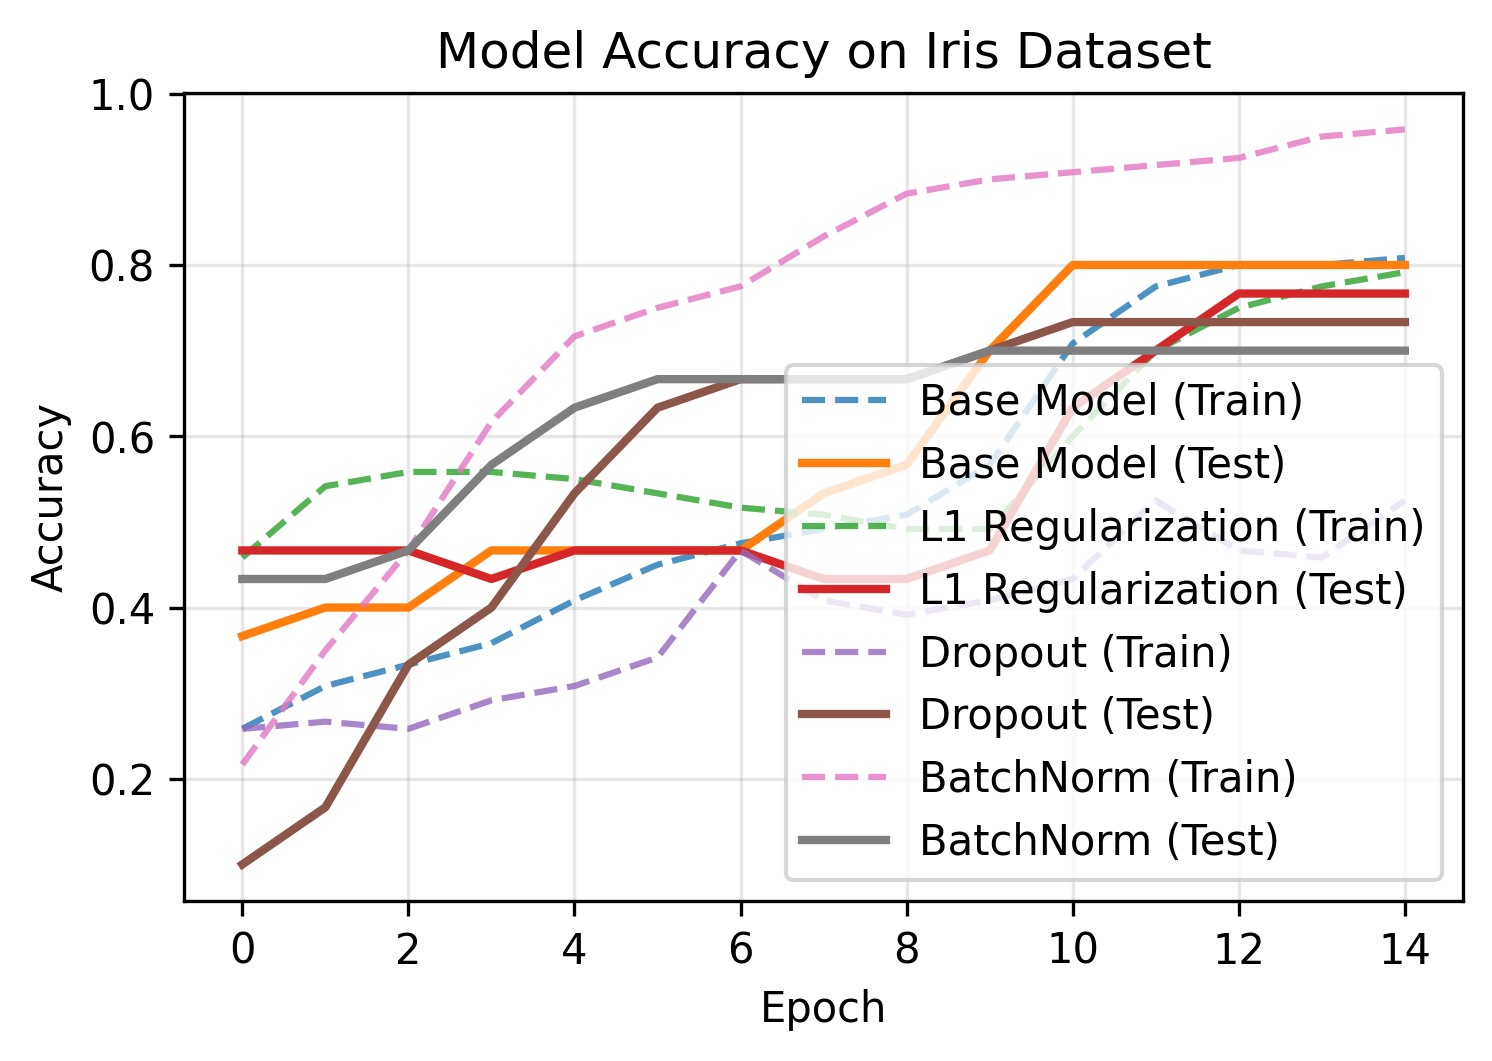
\includegraphics[keepaspectratio]{MarquezSalazarBrandon-Regularization_files/figure-pdf/cell-9-output-1.png}}

\subsubsection{Training and validation
loss}\label{training-and-validation-loss}

\texttt{}

\begin{Shaded}
\begin{Highlighting}[]
\ControlFlowTok{for}\NormalTok{ name, history }\KeywordTok{in}\NormalTok{ history\_dict.items():}
\NormalTok{    plt.plot(history.history[}\StringTok{\textquotesingle{}loss\textquotesingle{}}\NormalTok{], label}\OperatorTok{=}\SpecialStringTok{f\textquotesingle{}}\SpecialCharTok{\{}\NormalTok{name}\SpecialCharTok{\}}\SpecialStringTok{ (Train)\textquotesingle{}}\NormalTok{, linestyle}\OperatorTok{=}\StringTok{\textquotesingle{}{-}{-}\textquotesingle{}}\NormalTok{, alpha}\OperatorTok{=}\FloatTok{0.8}\NormalTok{)}
\NormalTok{    plt.plot(history.history[}\StringTok{\textquotesingle{}val\_loss\textquotesingle{}}\NormalTok{], label}\OperatorTok{=}\SpecialStringTok{f\textquotesingle{}}\SpecialCharTok{\{}\NormalTok{name}\SpecialCharTok{\}}\SpecialStringTok{ (Test)\textquotesingle{}}\NormalTok{, linewidth}\OperatorTok{=}\DecValTok{2}\NormalTok{)}
\NormalTok{plt.title(}\StringTok{\textquotesingle{}Model Loss on Iris Dataset\textquotesingle{}}\NormalTok{)}
\NormalTok{plt.ylabel(}\StringTok{\textquotesingle{}Loss\textquotesingle{}}\NormalTok{)}
\NormalTok{plt.xlabel(}\StringTok{\textquotesingle{}Epoch\textquotesingle{}}\NormalTok{)}
\NormalTok{plt.legend(loc}\OperatorTok{=}\StringTok{\textquotesingle{}upper right\textquotesingle{}}\NormalTok{)}
\NormalTok{plt.grid(}\VariableTok{True}\NormalTok{, alpha}\OperatorTok{=}\FloatTok{0.3}\NormalTok{)}

\NormalTok{plt.tight\_layout()}
\NormalTok{plt.show()}
\end{Highlighting}
\end{Shaded}

\pandocbounded{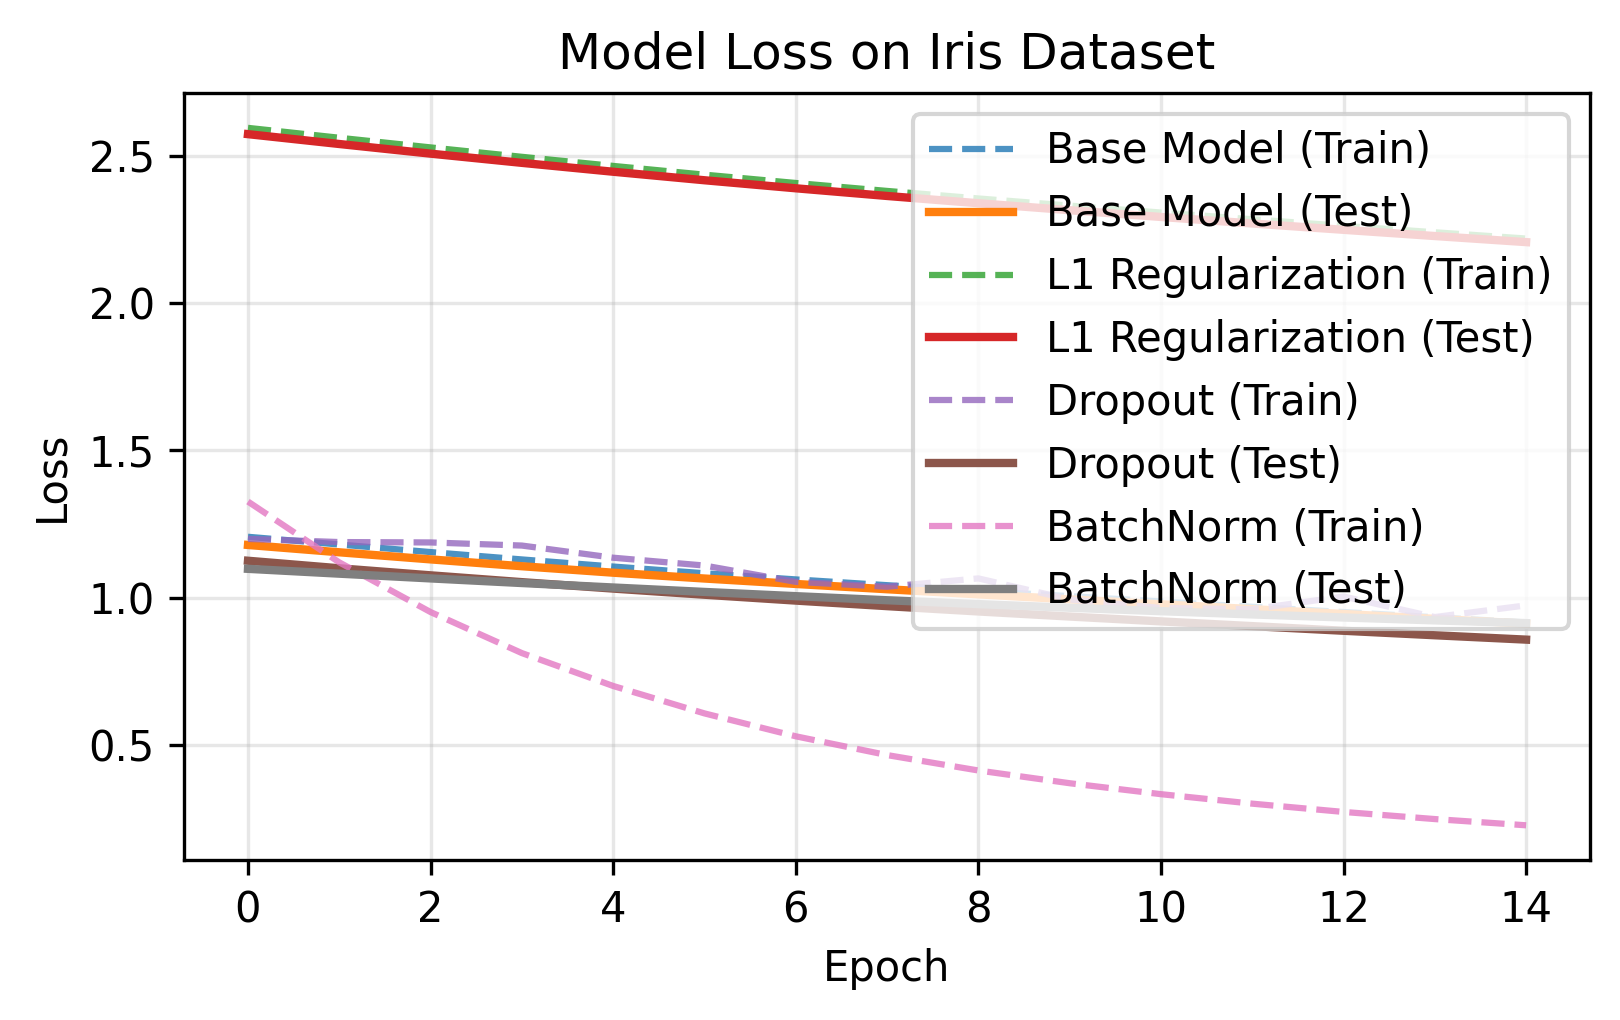
\includegraphics[keepaspectratio]{MarquezSalazarBrandon-Regularization_files/figure-pdf/cell-10-output-1.png}}

\subsubsection{Model comparison}\label{model-comparison}

Different models compared by parameters and size

\begin{Shaded}
\begin{Highlighting}[]
\BuiltInTok{print}\NormalTok{(}\StringTok{"}\CharTok{\textbackslash{}n}\StringTok{Model Complexity (Number of Trainable Parameters):"}\NormalTok{)}
\ControlFlowTok{for}\NormalTok{ name, model }\KeywordTok{in}\NormalTok{ models\_dict.items():}
\NormalTok{    total\_params }\OperatorTok{=}\NormalTok{ model.count\_params()}
    \BuiltInTok{print}\NormalTok{(}\SpecialStringTok{f"}\SpecialCharTok{\{}\NormalTok{name}\SpecialCharTok{\}}\SpecialStringTok{: }\SpecialCharTok{\{}\NormalTok{total\_params}\SpecialCharTok{:,\}}\SpecialStringTok{ parameters"}\NormalTok{)}
\end{Highlighting}
\end{Shaded}

\begin{verbatim}

Model Complexity (Number of Trainable Parameters):
Base Model: 2,499 parameters
L1 Regularization: 2,499 parameters
Dropout: 2,499 parameters
BatchNorm: 2,883 parameters
\end{verbatim}


\nocite{*}
\printbibliography



\end{document}
